\documentclass[11pt,a4paper]{article}
\usepackage[left=2cm,right=2cm,top=2cm,bottom=3cm]{geometry}
\usepackage{amsmath,amsfonts,amsthm,amssymb,varioref,times, commath}
\usepackage{gensymb}
\usepackage{tikz}
\usepackage{textcomp}
\usepackage{hyperref}
\hypersetup{
 colorlinks=true,
 linkcolor=blue,
 filecolor=magenta, 
urlcolor=cyan,
}
\usepackage{lipsum}
\usepackage{epigraph}
%to resume numbering in a list
\usepackage{enumitem}
%----- arrows 
\usepackage{extarrows}

%    differential equatiosn 
\usepackage{diffcoeff}   %\diff[2]{x}{y}


%%%%%%pour ecrire en français avec les accents
\usepackage[utf8]{inputenc}
\usepackage[T1]{fontenc}
\usepackage{lmodern} % load a font with all the characters
\usepackage{units}
%%%%%%%Image-related packages
\usepackage{wrapfig}
\usepackage{float, graphicx}
\graphicspath{ {./img/} }
\usepackage{subcaption}
\usepackage[export]{adjustbox}

%%%%%%%pour faire des cadres
\usepackage{xcolor}
\usepackage{tcolorbox}
\usepackage{framed}
\usepackage{mdframed}


%%%%%%%chemistry frmulae
\usepackage{chemfig}
\usepackage{chemformula}
\usepackage[version=4]{mhchem}

% -------------- Circuits -------------------
\usepackage[european, straightvoltages]{circuitikz}

% Title & headers
\usepackage[explicit]{titlesec}
% Raised Rule Command:
% Arg 1 (Optional) - How high to raise the rule
% Arg 2 - Thickness of the rule
\newcommand{\raisedrulefill}[2][0ex]{\leaders\hbox{\rule[#1]{1pt}{#2}}\hfill}
\titleformat{\section}{\Large\bfseries}{\thesection. }{0em}{#1\,\raisedrulefill[0.4ex]{1pt}}

% pour ecrire sur +sieurs colonnes
\usepackage{multicol}
\setlength{\columnseprule}{0pt}
\setlength{\columnsep}{60pt}
% Fusion de lignes de tableaux.
\usepackage{multirow}
% Position verticale des lettres dans la ligne de tableau.
\usepackage{array}

% physics -----------------------------------------------------------
\newcommand{\To}{\longrightarrow}
\newcommand{\gpl}{\; g\cdot L^{-1}}
\newcommand{\gpmol}{\; g\cdot mol^{-1}}
\newcommand{\mpl}{\; mol\cdot L^{-1}}
\newcommand{\mps}{\; m\cdot s^{-1}}
\newcommand{\rps}{\; rad\cdot s^{-1}}
\newcommand{\kph}{\; km\cdot h^{-1}}
\newcommand{\mpss}{\; m\cdot s^{-2}}
\newcommand{\Dt}{\Delta t}
\newcommand{\vv}{\vec{v}}
\newcommand{\va}{\vec{a}}
\newcommand{\vp}{\vec{p}}
\newcommand{\vf}{\vec{F}}
\newcommand*{\Vf}[1]{\overrightarrow{F_\ensuremath{{#1}}}}
\newcommand{\es}[1]{\cdot10^{#1}}
\newcommand{\eng}[1]{\textcolor{purple}{(= #1})}
\usepackage{harpoon}
%\newcommand*{\vect}[1]{\overrightharp{\ensuremath{#1}}}
\newcommand*{\Vect}[1]{\overrightarrow{\ensuremath{#1}}}
\newcommand{\pfd}[1]{\sum \vec{F}_{ext_{#1}} &= \od{\vp_{#1}}{t} = m\cdot\va_{#1}}
\newcommand{\C}{\degree C}
\newcommand{\Delt}{\Delta t}

% --- Circuits ------------
\newcommand{\bipole}[1]{
\begin{circuitikz} \draw
(0,0) to[ #1 ] (2,0); 
\end{circuitikz} {\hspace{5mm}}}

% Chimie ---------------------------------
\newcommand{\oxo}{\ce{H3O+}_{(aq)}}
\newcommand{\eau}{\ce{H2O}_{(\ell)}}
\newcommand{\OH}{\ce{HO-}_{(aq)}}
\newcommand{\AH}{\ce{AH}_{(aq)}}
\newcommand{\A}{\ce{A-}_{(aq)}}
\newcommand{\MnO}{\ce{MnO_4^{-}}}
\newcommand{\conc}[1]{\left[{#1}\right]}
\newcommand{\couple}[2]{\ce{#1/#2}}


% Environnements ------------------------
\newcounter{exo}
\newenvironment{exo}[1][]
{\refstepcounter{exo} \begin{shaded}\noindent $\triangleright \quad$\textbf{Exercice~\theexo. #1} } { \end{shaded}}
\newenvironment{eg}
{\begin{shaded} \textbf{Exemple:} } { \end{shaded}}

\newenvironment{defn}[1]
{\begin{leftbar}\noindent \textbf{Définition :\textit{ \quad #1}} } { \end{leftbar}}

%\newenvironment{rmrq}
%{\begin{shaded} \textbf{Remarque.\quad } \itshape } { \end{shaded}}
\newenvironment{rmrq}
{\begin{mdframed}[backgroundcolor=blue!10, linewidth=0pt] \textbf{Remarque.\quad } \itshape } { \end{mdframed}}

\newenvironment{python}
{\begin{shaded} \textbf{A faire en PYTHON}\\ \itshape } { \end{shaded}}

% Shading colour -----------------------------
\definecolor{shadecolor}{gray}{0.9}

\date{}
\author{}

\renewcommand*\contentsname{Résumé}









% Title & headers 
\usepackage{fancyhdr}
\pagestyle{fancy}
\fancyhf{}
\lhead{SciPhy : Terminale spé}
\rhead{$\chi $ - 3a : Acides \& Bases}
\chead{2020-28}
\rfoot{Page \thepage}
\lfoot{\textcopyright\; S Zayyani}
\renewcommand{\footrulewidth}{0.1pt}% default is 0pt

\title{\large Chimie - Chapitre 3a \\ \LARGE  Les Acides \& les Bases}



\setlength{\parindent}{0mm}
\setlength{\parskip}{2mm}

\setlength{\intextsep}{6pt}%
\setlength{\columnsep}{5pt}%

\begin{document}
\maketitle
\vspace{-1cm}
\begin{tcolorbox}[title=Notions de la classe de première à rappeler]
calcul d'un logarithme ; solvatation d'un proton libre dans l'eau ; Concentration molaire
%\tcblower
\end{tcolorbox}
\tableofcontents

\section{Acides \& Bases}
Nous avons vu une grande catégorie de réactions l'année dernière : les réactions d'oxydoréduction. Pour tout résumer en une phrase, les réactions rédox sont des réactions pendant lesquelles il y a un échange de un ou plusieurs électrons. Voici la raison pour laquelle l'étude des réaction rédox s'appelle de l'électrochimie. 

Nous allons maintenant aborder le ``revers de la médaille'' : les réactions où il y a un échange de protons entre les réactifs, c'est-à-dire les réactions acido-basiques. 

\subsection{Le pH}

\begin{defn}{pH }
\begin{itemize}
    \item L'acidité (ou la basicité) d'une solution dépend de la concentration des ions oxonium  $\oxo$ (i.e. protons libres associés aux molécules d’eau).
    \item Le $pH$ d'une solution est une mesure de l'acidité/basicité de la solution.
    \item Pour les solutions aqueuses diluées, le $pH$ dépend de la concentration des ions oxonium. Il est donné par la relation suivante : 
    \[  pH = -\log{[\oxo]} \quad \Longleftrightarrow \quad [\oxo] = 10^{-pH}\] 
    \item Le $pH$ est sans unité, et la concentration de la solution doit être exprimée en $\mpl$. 
\end{itemize}
\end{defn}

\begin{rmrq} Il y a deux choses à remarquer concernant cette définition du $pH$. Dans un premier temps, comme c'est souvent le cas, cette relation n'est valable que pour une certaine gamme de concentration, et sa validité diminue dans les concentrations trop élevées. Le deuxième point concerne la définition du $pH$. 

Dans l'intérêt de la rigueur, la définition est $pH = -\log{\dfrac{[\oxo]}{c^0}}$ où $c_0 = 1\mpl$ et s'appelle la \emph{concentration standard}. Ainsi le terme à l'intérieur de la fonction $\log$ est bien sans unité, comme le $pH$. 
\end{rmrq}

\begin{exo}
\begin{enumerate}
    \item Calculer le $pH$ des solutions de concentration en ions oxonium suivantes : 
    \begin{center}
      \begin{tabular}{c c}
        $1,0\es{-2} \mpl$ \quad ;  & $5,0\es{-3} \mpl$ \\
        $4,3\es{-3} \mpl$ \quad ; & $2,0\es{-8} \mpl$ \\
    \end{tabular}  
    \end{center}
    \item Calculer la valeur approchée de la concentration en ion oxonium des solutions des $pH$ suivants : $1,5 \quad ; \quad 3,0 \quad ; \quad 2,2 \quad ; \quad 7,7$.
    \item Ecrire un encadrement de la valeur de la concentration en ions oxonium de la solution de $pH = 1,5$ si le $pH$ est donné à $\pm 0,1$ unité de $pH$. Est-il utile de donner trois chiffre significatifs? 
\end{enumerate}    

\textbf{Solution : }
\begin{enumerate}
    \item 
    
    %\begin{center}
    \begin{tabular}{c||c|c|c|c}
         $[\oxo](\mpl)$ & $1,0\es{-2}$  & $5,0\es{-3} $ & $4,3\es{-3}$ & $2,0\es{-3} $ \\ \hline
         $pH$ &  $2,0$ & 2,3 & 2,4 & 7,7 
    \end{tabular}    
    \vspace{0.5cm}
   % \end{center}
    \item     
    
    %\begin{center}
    \begin{tabular}{c||c|c|c|c}
         $pH$ &  1,5 & 3,0 & 2,2 & 7,7  \\ \hline
         $[\oxo](\mpl)$ & $3,2\es{-2}$  & $1,0\es{-3} $ & $6,3\es{-3}$ & $2,0\es{-8} $         
    \end{tabular}    
    %\end{center}
    \vspace{0.5cm}
    \item Selon l'énoncé, l'encadrement demandé correspond à $1,4 < pH < 1,6$ et donc 
       \begin{align*}
        [\oxo] &= 10^{-1,4} = 3,98\es{-2}\mpl \\
        [\oxo] &= 10^{-1,6} = 2,51\es{-2}\mpl
    \end{align*}    
    ainsi l'encadrement des concentration devient (en respectant les chiffres significatifs) : 
    $$ 2,5\es{-2}\mpl < pH < 4,0 \es{-2}\mpl$$
\end{enumerate}
\end{exo}	

\subsection{Acides \& Bases}	

C’est en classe de $3^e$ que l’on entend parler pour la première fois des acides et des bases, lors de l'étude d’\textit{attaque des métaux par des acides}. 
On peut donner comme exemple la réaction entre l’acide chlorhydrique $\ce{HC\ell}$ et le métal cuivre $\ce{Cu}$.  Les produits de cette réaction étaient l’ion métallique $\ce{Cu^2+}$ (cuivre II) et l’ion chlorure $\ce{Cl-}$ (mis en évidence grâce au test de \ce{NaOH}), et un gaz explosif (le dihydrogène $\ce{H2}$  ).  Trouvons d’abord le bilan de cette réaction, puis, son équation-bilan : 
\[\ce{HC\ell}  +  \ce{Cu -> 2 C\ell- + H2 + Cu^2+} \]

Ici, chaque atome de cuivre réagit avec deux molécules d’acide.  Si l'on voyait ce qui se passe à l'échelle des atomes dans les molécules, on verrait que lors de cette réaction deux ions d'hydrogène provenant de l’acide chlorhydrique sont libérés, et puis sont transférés à l'atome de cuivre.  Ce transfert de protons est bien ce qui caractérise une réaction acido-basique. 

\begin{defn}{Acide \& Base}
\begin{itemize}
    \item Une réaction acido-basique est caractérisée par un \textbf{transfert de proton $\ce{H+}$} entre un acide et une base.
    \item Un \textbf{acide} est une entité chimique capable de \textbf{libérer/céder un proton}  : $\ce{Acide} \To \ce{X} + \ce{H+}$
    \item Un \textbf{base} est une entité chimique capable de \textbf{capter un proton}  : $\ce{Base} + \ce{H+} \To \ce{Y}$
\end{itemize}    
\end{defn}

\section{Le couple acide/base}

Désormais, on utilise la convention simplifiée suivante : $\ce{AH}$ représente un acide, et $\ce{A-}$ représente une base.  Si l'on réécrit la définition d'un acide nous avons : $\ce{AH} \To \ce{A-} + \ce{H+}$. 
Mais la réaction inverse serait :   $\ce{A-} + \ce{H+} \To \ce{AH}$. Mais on voit clairement que cette dernière correspond à la définition d’une base, où $ \ce{A-}$ est la base :$\ce{A-}$ est simplement la base associée à l’acide $\ce{AH}$, ou plus précisément $\ce{A-}$  est la \textbf{base conjuguée} de l’acide $\ce{AH}$.  

\begin{defn}{Couple acide/base}
\begin{itemize}
    \item Deux entités chimiques constituent un couple acide/base s’il est possible \textbf{de passer de l’une à l’autre par perte ou gain d’un proton}
    \item L’acide est noté AH, la base $\ce{AH}$  et le couple $\ce{A-} / \ce{A-}$(l’\textbf{acide est toujours noté en premier})
    \item $\ce{A-}$ est la base conjuguée de l’acide $\ce{AH}$, et $\ce{AH}$ est l’acide conjugué de la base $\ce{A-}$.
    \item Comme avec les réaction rédox, il existe une notation compacte pour ces demi-équations acido-basiques, où $`` = "$ signifie les deux réactions opposées du couple: 
    $$\ce{AH} = \ce{A-} + \ce{H+} $$ 
\end{itemize}
\end{defn}

Voici un exemple de quelques couples acide/bases que l'on observe très souvent : 

\begin{figure}[ht]
\centering
\begin{subfigure}{.53\textwidth}
  \centering
  % include first image
  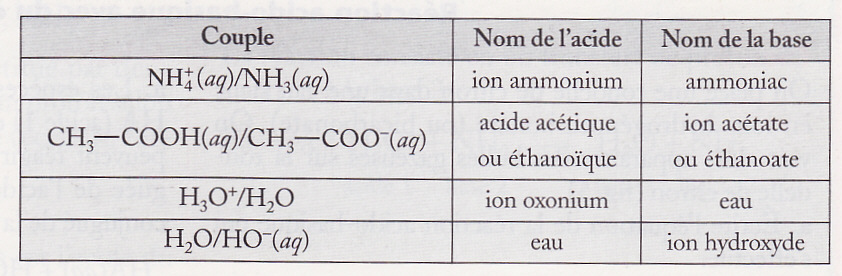
\includegraphics[width=\linewidth]{imgs/c3/tableAB.jpg}  
\end{subfigure}
\begin{subfigure}{.46\textwidth}
  \centering
  % include second image
  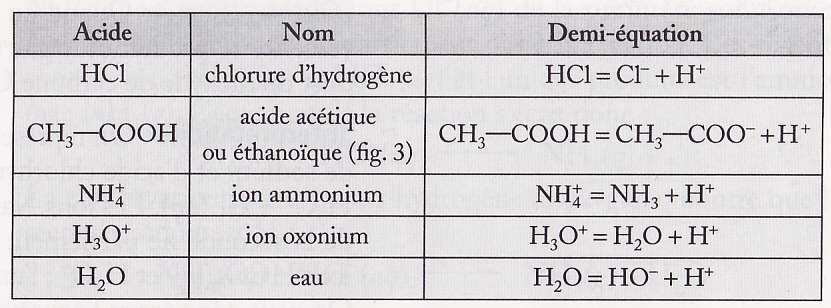
\includegraphics[width=\linewidth]{imgs/c3/tableACIDES.jpg}  
\end{subfigure}
\caption{Quelques exemples des couples acide/base.}
\end{figure}

Si l'on regarde le bas du tableau précédent, on constate que l'eau est listée comme base mais aussi comme acide, et dans deux couples différents, une fois avec l'oxonium, et une fois avec l'ion hydroxyle: 

\begin{itemize}
    \item Dans le couple $ \oxo/\eau \quad$ : $\quad \oxo = \eau + \ce{H+}$
    \item Dans le couple $ \eau / \OH \quad $ : $\quad \eau = \OH + \ce{H+}$
\end{itemize}

Dans le premier cas, l’eau est la base, le récipient du proton.  Tandis que dans le deuxième cas, l’eau est l’acide, car c’est elle qui libère le proton.  On dit que l’eau un \textbf{ampholyte (adj. amphotère)}\eng{Amphoteric compound} ;  c'est-à-dire une espèce chimique qui appartient à deux couples acide/base, $ \oxo/\eau$ et $ \eau / \OH$.  

Elle est une espèce qui se comporte comme un acide ou une base selon la situation (en présence d’une base, comme un acide ; en présence d’un acide, comme une base). C'est le cas de beaucoup d'autres espèces chimiques. En effet, dès qu'il s'agit d'un \emph{poly-acide} (acide capable de céder plusieurs protons, comme l'acide sulfurique ou acide phosphorique) il y a au moins un ampholyte. 

\begin{eg} % ---------------- exemple amhpolyte-------------
\begin{itemize}
    \item Acide sulfurique : $\ce{H2SO4}$ : 
    \begin{itemize}
        \item Première acidité : $\ce{H2SO4} = \ce{HSO4-} + \ce{H+}$
        \item Deuxième acidité : $\ce{HSO4-} = \ce{SO4^2-} + \ce{H+}$
    \end{itemize}
    Ici l'ion hydrogénosulfate $\ce{HSO4-}$ est un ampholyte. 
    \item Acide phosphorique : $\ce{H3PO4}$ : 
    \begin{itemize}
        \item Première acidité : $\ce{H3SO4} = \ce{H2PO4-} + \ce{H+}$
        \item Deuxième acidité : $\ce{H2PO4-} = \ce{HPO4^2-} + \ce{H+}$
        \item Troisième acidité : $\ce{HPO4^2-} = \ce{PO4^3-} + \ce{H+}$
    \end{itemize}    
    Ici les ions $\ce{HPO4^2-}$ et $\ce{H2PO4-}$ sont amphotères. 
\end{itemize}
\end{eg}

\section{Réaction acido-basique}% --------------- SECTION------------

\begin{defn}{Réaction acido-basique}
\begin{itemize}
    \item Lors d'une réaction acido-basique il y a un \textbf{échange de proton(s)}\eng{proton exchange} entre les deux réactifs. 
    \item Une réaction acido-basique fait \textbf{intervenir deux couples acide/base}. 
    \item Réaction est, forcément, \textbf{entre l'acide d'un couple et la base de l'autre}. 
\end{itemize}
\end{defn}

Considérons deux couples d'acide/base quelconque : $\ce{A1H}/\ce{A1-} \quad $ et $\quad \ce{A2H}/\ce{A2-}$. Les demi-équations associées sont : 
$$ \ce{A1H} = \ce{A1-} + \ce{H+}\quad \text{et}\quad \ce{A2H} = \ce{A2-} + \ce{H+}$$

Afin d'avoir un échange de protons il faut une espèce qui cède le proton (l'acide) et l'autre qui le capte (la base), c'est-à-dire, sans plus d'information, il y a deux possibilités pour ces deux couples : soit l'acide du premier couple réagit avec la base du deuxième couple, soit c'est la base du premier couple avec l'acide du deuxième couple. 

Prenons le premier cas (un seul cas suffit, comme illustration). Les démi-réactions seront donc : 
\begin{align*}
    \ce{A1H} &\To \ce{A1-} + \ce{H+} \\
    \ce{A2-} + \ce{H+} &\To \ce{A2H}
\end{align*}

La réaction finale, c'est-à-dire la réaction acido-basique entre les deux couples est la somme de ces deux demi-réactions : 

$$\ce{A1H} + \ce{A2-} + \ce{H+} \To \ce{A2H} + \ce{A1-} + \ce{H+} $$

Il y a un proton $\ce{H+}$ des deux côtés, et donc la réaction simplifiée est  : 

$$\ce{A1H} + \ce{A2-} \To \ce{A2H} + \ce{A1-} $$

\begin{rmrq}
Dans un sens, le proton transféré ne figure pas dans l’équation chimique. Mais dans un autre sens, cette équation montre le transfert d’un proton de l’acide $\ce{A1H}$ à la base $\ce{A_2^-}$. 

Dans les demi-équations, on utilise = mais dans la réaction a/b on utilise plutôt → car il s’agit d’une véritable réaction chimique. 

\end{rmrq}

\begin{exo}
Indiquer en dessous de l’équation l’acide et la base pour les réactifs et les produits, et compléter l’équation. 
\begin{enumerate}
    \item $\ce{CH3COOH}_{(aq)} + \OH \To $
    \item $\ce{C6H5COO-}_{(aq)} + \oxo \To$
    \item $\oxo + \OH \To $
    \item $\ce{NH3}_{(aq)} + \eau \To $
    \item $\ce{NH4+}_{(aq)} + \eau \To $
\end{enumerate}
\end{exo}

\section{Réaction avec l'eau}% --------------- SECTION------------

Nous allons maintenant se poser la question du comportement des acides dans l'eau, surtout car la plupart des solutions acides ou basiques sont des solutions aqueuse, et donc le comportant d'un acide ou d'une base est primordiale pour la compréhension de la suite. 


\subsection{Autoprotolyse de l'eau}
  
Mais d'abord on peut se poser la question de la nature acide ou basique de l'eau. On peut répondre à cette question si on donne la(les) demi-équation(s) contenant de l’eau.  Il y en a deux :

\begin{itemize}
    \item Couples $\ce{H3O+}/\ce{H2O}$ dont la demi-équation :$\ce{H3O+} = \ce{H2O} + \ce{H+}$
    \item Couple $\ce{H2O} / \ce{H2O} $ dont la demi-équation : $\ce{H2O} = \ce{HO-} + \ce{H+}$
\end{itemize}
	
On voit donc que la molécule d'eau est amphotère. Tournons-nous maintenant vers une réaction très importante qui dépend, justement, de ce caractère amphotère de l'eau. 

\begin{defn}{L'autoprotolyse de l'eau\eng{self-ionization of water}}
\begin{itemize}
    \item La réaction acido-basique qui a lieu \textbf{entre deux molécules d’eau}, dans toute solution aqueuse, est appelée réaction d’autoprotolyse de l’eau.  Elle est représentée par l’équation suivante : 
    \begin{align*}
        \eau + \eau  &\rightleftharpoons \OH + \oxo \\
        2\eau  &\rightleftharpoons \OH + \oxo
    \end{align*}
    \item C’est une réaction très \textbf{limitée} 
\end{itemize}
\end{defn}

\begin{defn}{Produit ionique de l’eau}
\begin{itemize}
    \item Le produit ionique de l’eau, noté $K_e$, est donnée par : 
    \[ K_e = [\oxo][\OH]\]
    \item À une température donnée, le produit ionique de l’eau a la même valeur pour toute solution aqueuse. À température ambiante (i.e. $25\degree C$) $K_e = 1,0\es{-14}$. 
\end{itemize}
\end{defn}

\begin{exo}
Le $pH$ d’une solution aqueuse d’un acide $\ce{AH}$ est égal à $3,5$ à $25\degree C$. À partir de la définition du $pH$ donner la concentration de la solution en ions oxonium. En déduire la concentration de la solution en ions hydroxyde. 
\vspace{3cm}
\end{exo}
 
\begin{exo}
Les solutions basiques sont souvent riches en ions hydroxyde. Si la concentration en ions hydroxyde $[\OH]_{éq}$  d’une solution à l’équilibre est connue, on peut déterminer le $pH$ en utilisant le produit ionique de l’eau. Déterminer l’expression du $pH$ en fonction de $K_e$ et de $[\OH]_{éq}$.  
\vspace{3cm}
\end{exo} 


\end{document}

